\documentclass[english]{maciarticle}
%\documentclass[spanish]{maciarticle}
%% If your article is written in spanish you have to write the option "spanish"

\usepackage{amsmath,amsbsy,amscd,amssymb,graphicx, epsfig,color, float}


%%%%%%%%%%%%%%%%%%%%%%%%%%%%%%%%%%%%%%%%%%%%%
\begin{document}

\title{Argentine Association for Industrial, Computational and Applied Mathematics. Model Article}

\author[$\flat$]{Alan Matys}
\author[$\dag$]{Federico Rodriguez}
\affil[$\flat$]{Universidad del CEMA,
\textcolor{blue} {alan.matys92@gmail.com, federico.m.rodriguez.h@gmail.com}}


 \maketitle


\begin{abstract}This article is intended to tackle the portfolio-building problem by framing it as a budget allocation challenge, balancing expected returns and risk. Traditional methods like the Critical Line Algorithm (CLA) face diversification limitations. To address this, Hierarchical Risk Parity (HRP) offers a more structured approach, clustering correlated assets and assigning weights top-down. By leveraging the covariance matrix, HRP enhances diversification and aligns with real-world portfolio management practices. This methodology will be applied in the cryptocurrency domain to optimize asset allocation and risk management.
\end{abstract}
\begin{keywords}
Hierarchical Risk Parity, Risk-based asset allocation, Cryptocurrency, Portfolio Optimization
\end{keywords}
\begin{mathsubclass}
21A54 - 55P54
\end{mathsubclass}


{\thispagestyle{empty}} %DON`T DELETE THIS LINE



%%===============================
\section{Introduction}
%%===============================


\medskip

The portfolio construction problem can be framed as a budget allocation challenge, where each point in the allocation space represents a portfolio with different asset weightings. This problem is traditionally modeled in terms of expected return and risk, understood as the deviation of asset returns.

In a Capital Asset Pricing Model (CAPM) framework, portfolio optimization follows two main objectives:

\begin{itemize}
    \item Given a fixed risk level, maximize return.
    \item Given a target return, minimize associated risk.
\end{itemize}

For each portfolio, the portfolio return is a random variable, composed of the weighted sum of individual asset returns:


\[
R_p = \sum_{i=1}^N W_i R_{A_i}
\]

where:

\begin{itemize}
    \item \(R_p\): Portfolio return
    \item \(N\): Total number of assets in the portfolio
    \item \(A_i\): Asset \(i\)
    \item \(R_{A_i}\): Return of asset \(A_i\)
    \item \(W_i\): Budget weight assigned to asset \(A_i\), with \(\sum_{i=1}^N W_i = 1\).
\end{itemize}

A key challenge in this approach is the dependence on unobservable parameters. The mean and variance} of asset returns are population characteristics, which are unknown and can only be estimated from historical data within a given time window.

One of the traditional methods for portfolio optimization is the Markowitz Critical Line Algorithm (CLA), which solves the allocation problem by minimizing variance subject to return estimates over a defined time window. While the algorithm provides a theoretically optimal solution, it has both advantages and disadvantages:

\begin{itemize}
    \item \textbf{Pros:} Ensures weight convergence after a finite number of steps.
    \item \textbf{Cons:} Prone to instability, high concentration in specific assets, and potential underperformance.
\end{itemize}

Moreover, CLA requires inverting the variance-covariance matrix, a process that can be straightforward but, depending on the matrix structure, may lead to numerical instability and unreliable results.

Risk-based asset allocation methods address some of the challenges faced by the \textbf{CLA}. The goal is to diversify the portfolio based on information contained in the \textbf{covariance matrix}.

This article explores the application of \textbf{HRP in the cryptocurrency domain} one of the main risk based approaches. This is done by leveraging its ability to enhance diversification while addressing estimation uncertainty in risk and return parameters.

\section{HRP Portfolio Building}
The Hierarchical Risk Parity (HRP) approach aims to diversify the portfolio based on information contained in the covariance matrix Unlike traditional optimization methods, HRP introduces a hierarchical allocation structure that offers several advantages:

\begin{itemize}
    \item Weights are assigned hierarchically, grouping highly correlated assets before distributing weights within each group.
    \item Similar assets receive allocations first, followed by further subdivisions.
    \item Weights are assigned in a top-down manner, mirroring how many portfolio managers construct their portfolios.
\end{itemize}

A key advantage of HRP is its ability to function even when the covariance matrix is singular or lacks a well-defined inverse. This is achieved through a structured three-step process:

\subsection{Hierarchical Clustering}
The first step involves identifying clusters of assets based on their correlation matrix. By grouping highly correlated assets together, HRP constructs a hierarchical representation of the asset relationships.

\subsection{Quasi-Diagonalization}
Once clusters are identified, the next step is to reorder them based on their risk profile. This process ensures that assets with distinct risk characteristics are positioned effectively within the portfolio structure.

\subsection{Recursive Bisection}
The final step involves a recursive bisection process, where weights are assigned in a disaggregated manner. Instead of directly optimizing the covariance matrix inversion, HRP distributes weights progressively across the hierarchy, ensuring a stable and diversified allocation.

\vspace*{.25cm}


\subsection{Hierarchical Clustering}

The first step in HRP is the construction of a hierarchical clustering structure based on asset correlations. This process begins by computing a distance matrix derived from the correlations of \(N\) assets.

The correlation matrix is defined as:

\[
\rho = \left( \rho_{i,j} \right)_{i,j=1,...,N}
\]

where each element \(\rho_{i,j}\) represents the correlation between asset \(X_i\) and asset \(X_j\):

\[
\rho_{i,j} = \rho[X_i, X_j].
\]

Since the correlation matrix is bounded within \([-1,1]\), its scale does not affect the clustering process.

From this correlation matrix, we construct a distance metric to measure the dissimilarity between asset pairs. The metric is defined as:

\[
d : (X_i, X_j) \subseteq \mathcal{B} \to \mathbb{R} \in [0, 1], \quad d_{i,j} = d[X_i, X_j] = \sqrt{\frac{1}{2}(1 - \rho_{i,j})}.
\]

where \(\mathcal{B}\) represents the Cartesian product of asset pairs.

This transformation ensures that assets with high correlations are placed closer together in the hierarchical structure, forming the basis for further steps in the HRP allocation process.

With the previously computed distance matrix, we calculate the **Euclidean distances** between the columns of the matrix:

\[
\tilde{d} : (D_i, D_j) \subseteq \mathcal{B} \to \mathbb{R} \in [0, \sqrt{N}], \quad \tilde{d}_{i,j} = \tilde{d}[D_i, D_j] = \sqrt{\sum_{n=1}^N (d_{n,i} - d_{n,j})^2}.
\]

This results in \(\tilde{d}_{i,j}\) being a function of the entire correlation matrix, rather than just an individual correlation pair.

Finally, assets are grouped based on the final matrix using a **linkage criterion**, determining the hierarchical structure necessary for the next steps of the HRP process.

\subsection{Quasi-Diagonalization}

In this step, the matrix is reorganized such that rows and columns are arranged so that the largest values in the distance matrix are grouped along the diagonal.

Based on the clusters identified in the previous step, we reorder the matrix so that similar assets are positioned closer together, while uncorrelated or negatively correlated assets are placed farther apart. This structured ordering allows for a clearer representation of asset relationships and improves the stability of subsequent calculations.

As we move away from an asset’s cluster, correlations decrease, reinforcing the separation of distinct investment groups. By achieving a **quasi-diagonal structure**, this step significantly enhances the efficiency of further computations, particularly in weight allocation and portfolio construction.

\subsection{Recursive Bisection}

Using the quasi-diagonalization from the previous step, we now determine the **optimal portfolio allocation by applying the Inverse Variance Portfolio (IVP) method within each group. 

The IVP approach assigns portfolio weights inversely proportional to the variance of each asset, ensuring a risk-balanced allocation. The recursive bisection process follows these steps:

\begin{itemize}
    \item First, allocate weights to each major group identified in the clustering step.
    \item Then, recursively divide the assigned weights within each subgroup.
    \item Continue subdividing until further partitioning is no longer possible.
\end{itemize}

By iteratively splitting and distributing weights, this method ensures a stable and diversified allocation, avoiding over-concentration in specific assets. The recursive approach allows HRP to dynamically adjust portfolio weights while maintaining an optimal risk structure.


\section{Results and Evaluation Methodology}

The proposed method will be tested and compared against other portfolio allocation techniques, namely the Inverse Variance Portfolio (IVP) and the Minimum Variance Portfolio (MVP). In addition to these benchmarks, the strategy will also be evaluated against simple BTC holding and **ETH holding for the entire backtesting period.

For this analysis, the backtesting period spans two years, from \textbf{January 1, 2021, to December 31, 2023}.

\subsection{Comparison Scenarios}

The methodology will be assessed under two distinct scenarios:

\begin{itemize}
    \item \textbf{Static Portfolio Allocation}: Based on the initial data, portfolio weights will be assigned once at the beginning of the backtesting period, with no reweighting throughout the entire duration.
    \item \textbf{Weekly Rebalancing}: The best-performing method from the static allocation scenario will be compared against the three methodologies under a **weekly rebalancing** strategy.
\end{itemize}

\subsection{Evaluation Metrics}

To evaluate the performance of each portfolio strategy, the following metrics will be computed:

\begin{itemize}
    \item \textbf{Total Return (\%)}: The overall percentage gain or loss over the backtesting period.
    \item \textbf{Annualized Volatility (\%)}: Measures the standard deviation of returns on an annual basis.
    \item \textbf{Sharpe Ratio}: Evaluates risk-adjusted returns by comparing excess returns over the risk-free rate relative to volatility.
    \item \textbf{Sortino Ratio}: Similar to the Sharpe Ratio but only considers downside risk.
    \item \textbf{Maximum Drawdown (\%)}: The largest peak-to-trough decline in portfolio value during the period.
    \item \textbf{Calmar Ratio}: The return-to-risk measure comparing total return to maximum drawdown.
\end{itemize}

These metrics will provide a comprehensive assessment of the risk-adjusted performance and robustness of the HRP strategy in comparison to other allocation methods.

\subsection{Final Results}

In this section, we present the results for both portfolio allocation scenarios, focusing on Cumulative Returns and Metrics Evaluation.

\subsubsection{Static Portfolio Allocation Results}

\begin{figure}[h]
    \centering
    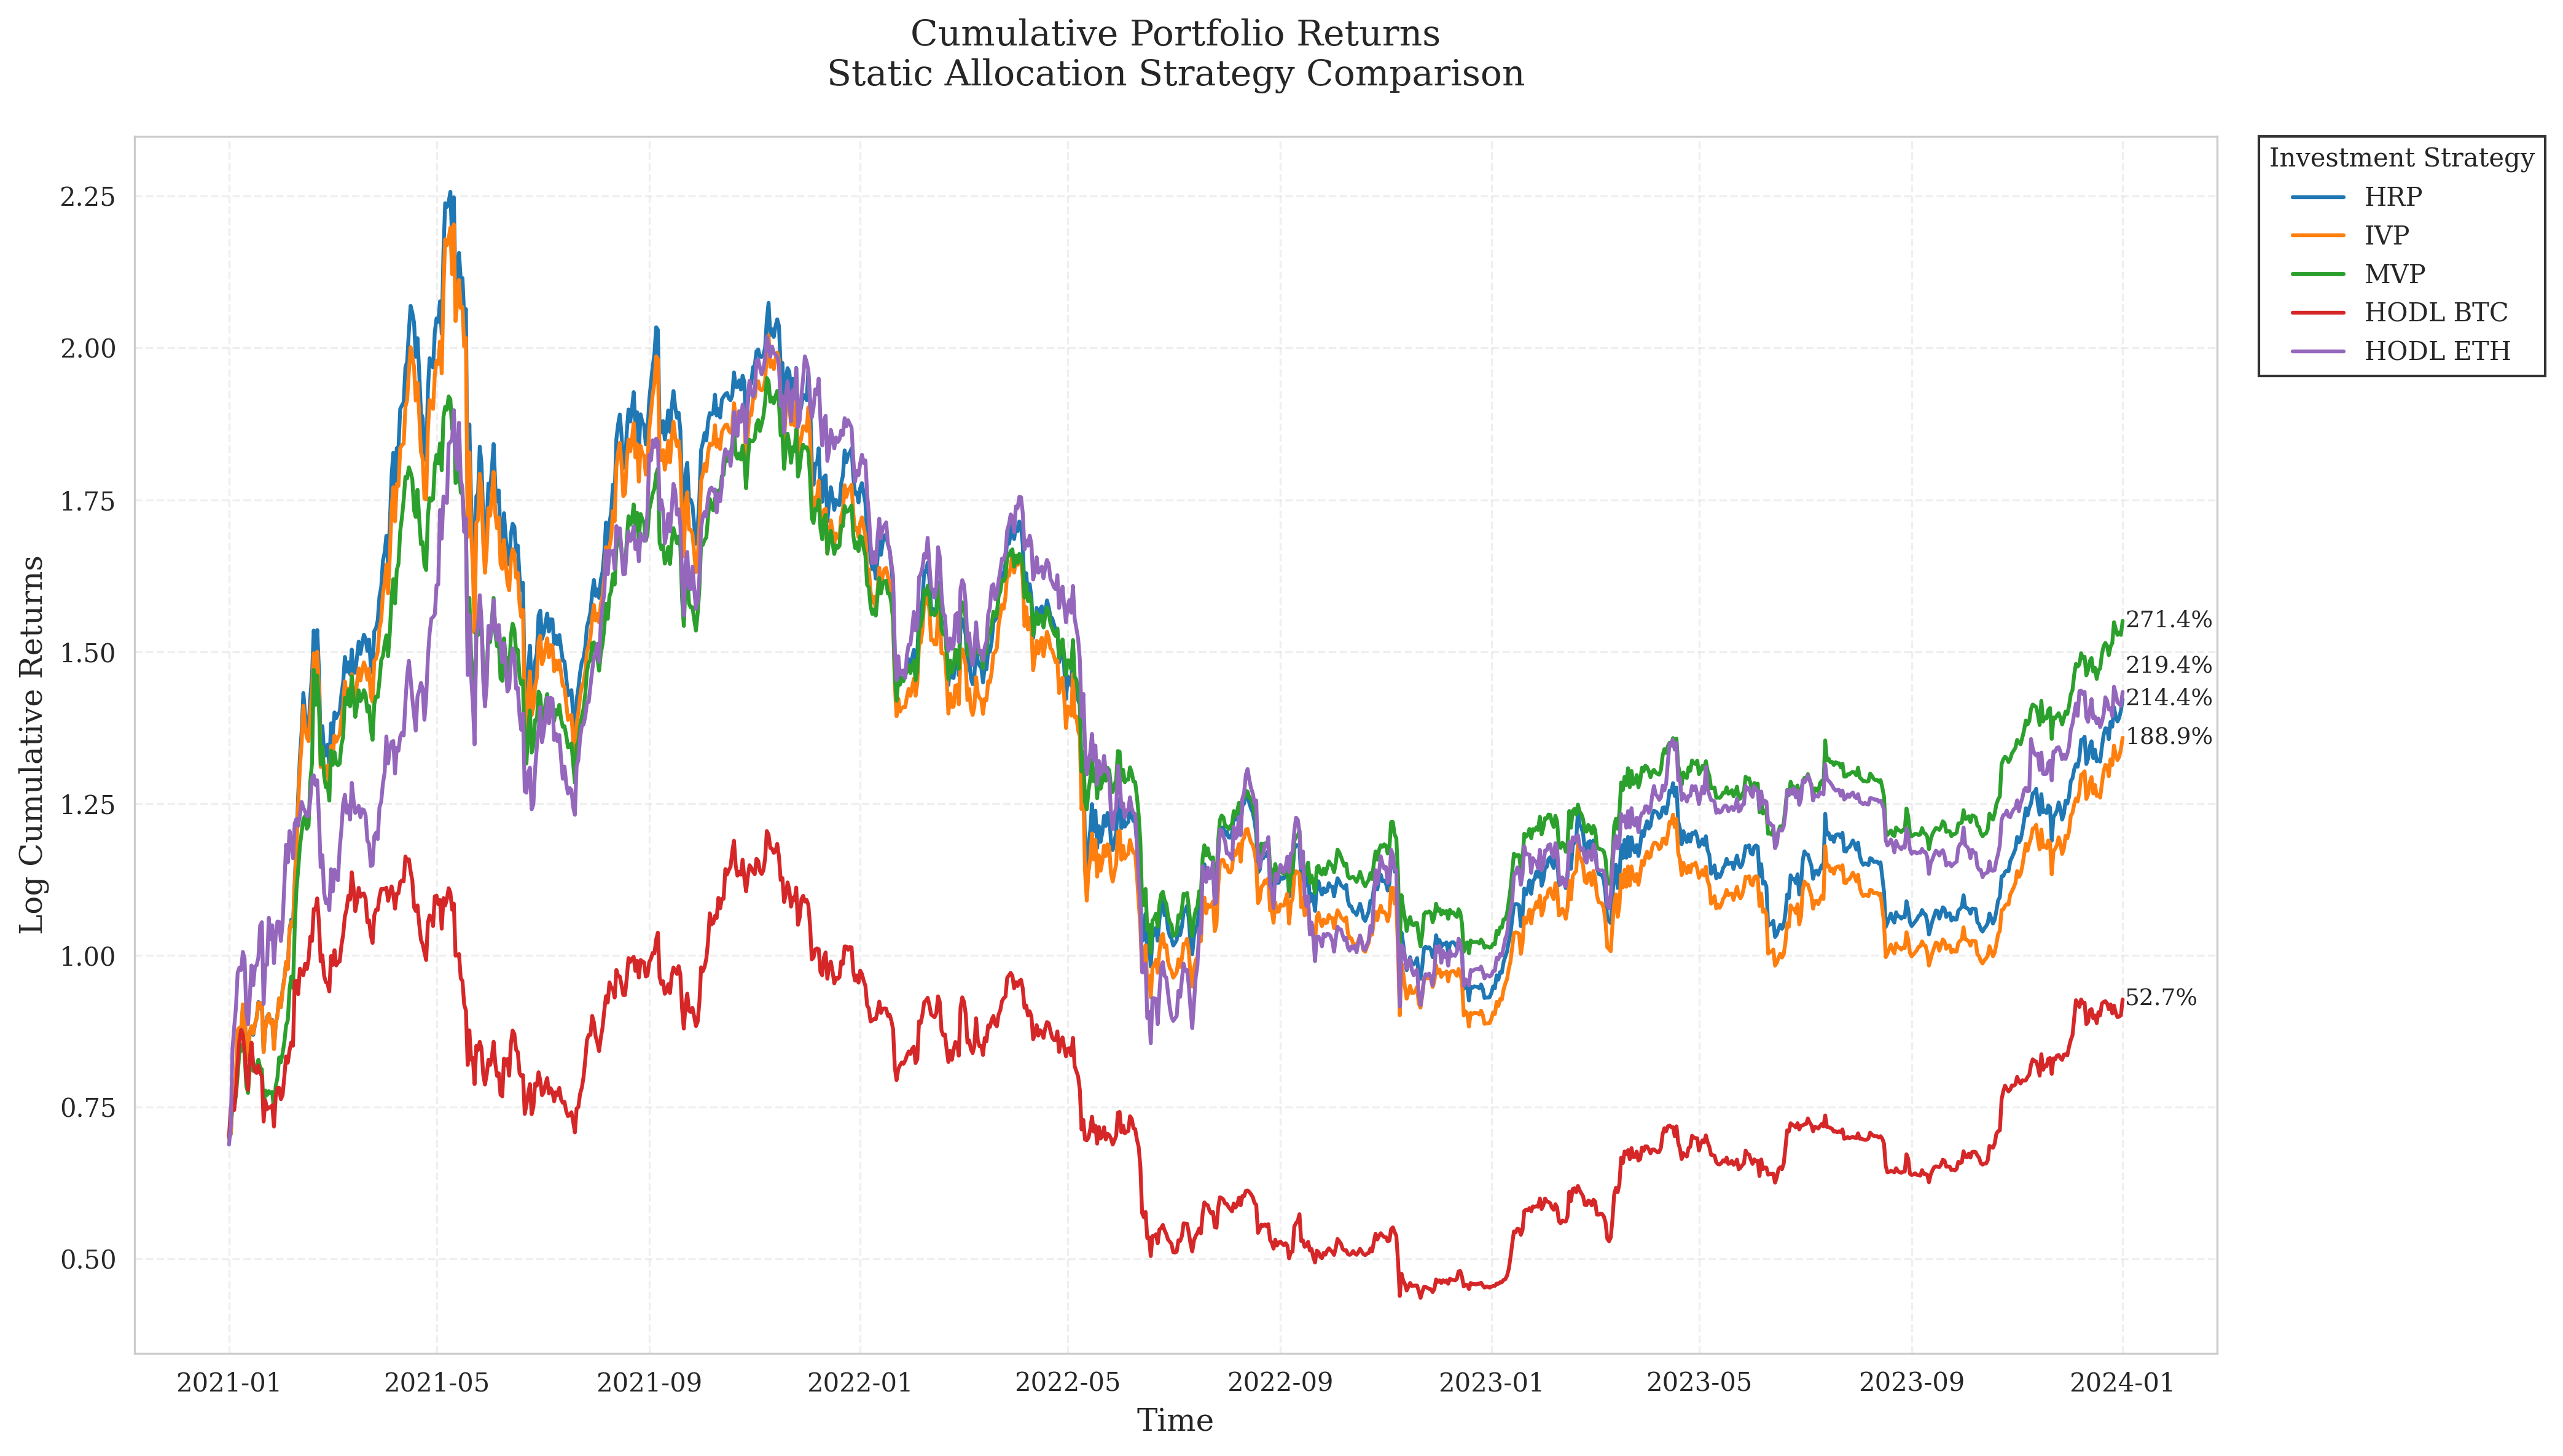
\includegraphics[width=0.7\textwidth]{static_cumulative_returns.png}
    \caption{Cumulative Returns for Static Portfolio Allocation.}
    \label{fig:static_cum_returns}
\end{figure}

\begin{figure}[h]
    \centering
    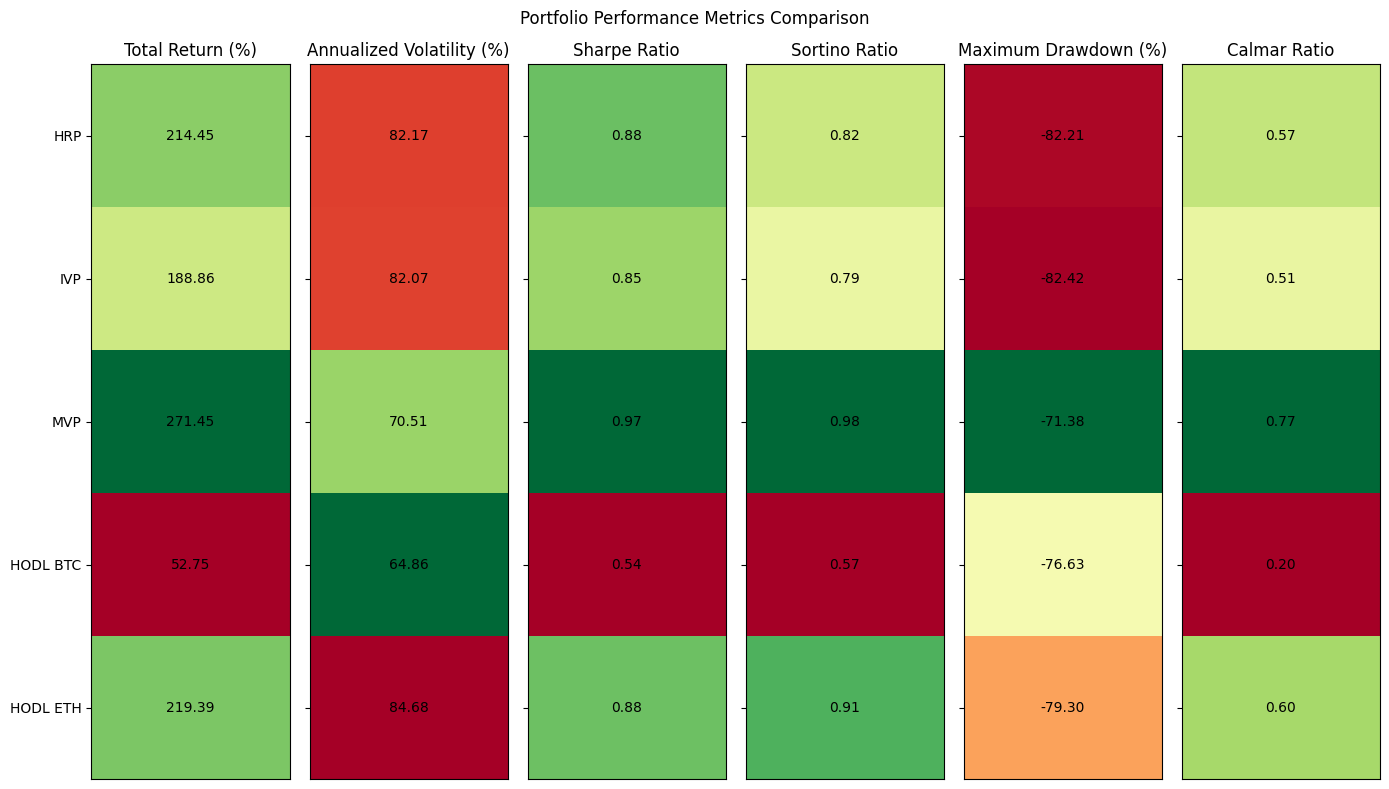
\includegraphics[width=0.7\textwidth]{static_metrics_evaluation.png}
    \caption{Metrics Evaluation for Static Portfolio Allocation.}
    \label{fig:static_metrics}
\end{figure}

\subsubsection{Weekly Rebalancing Results}

\begin{figure}[h]
    \centering
    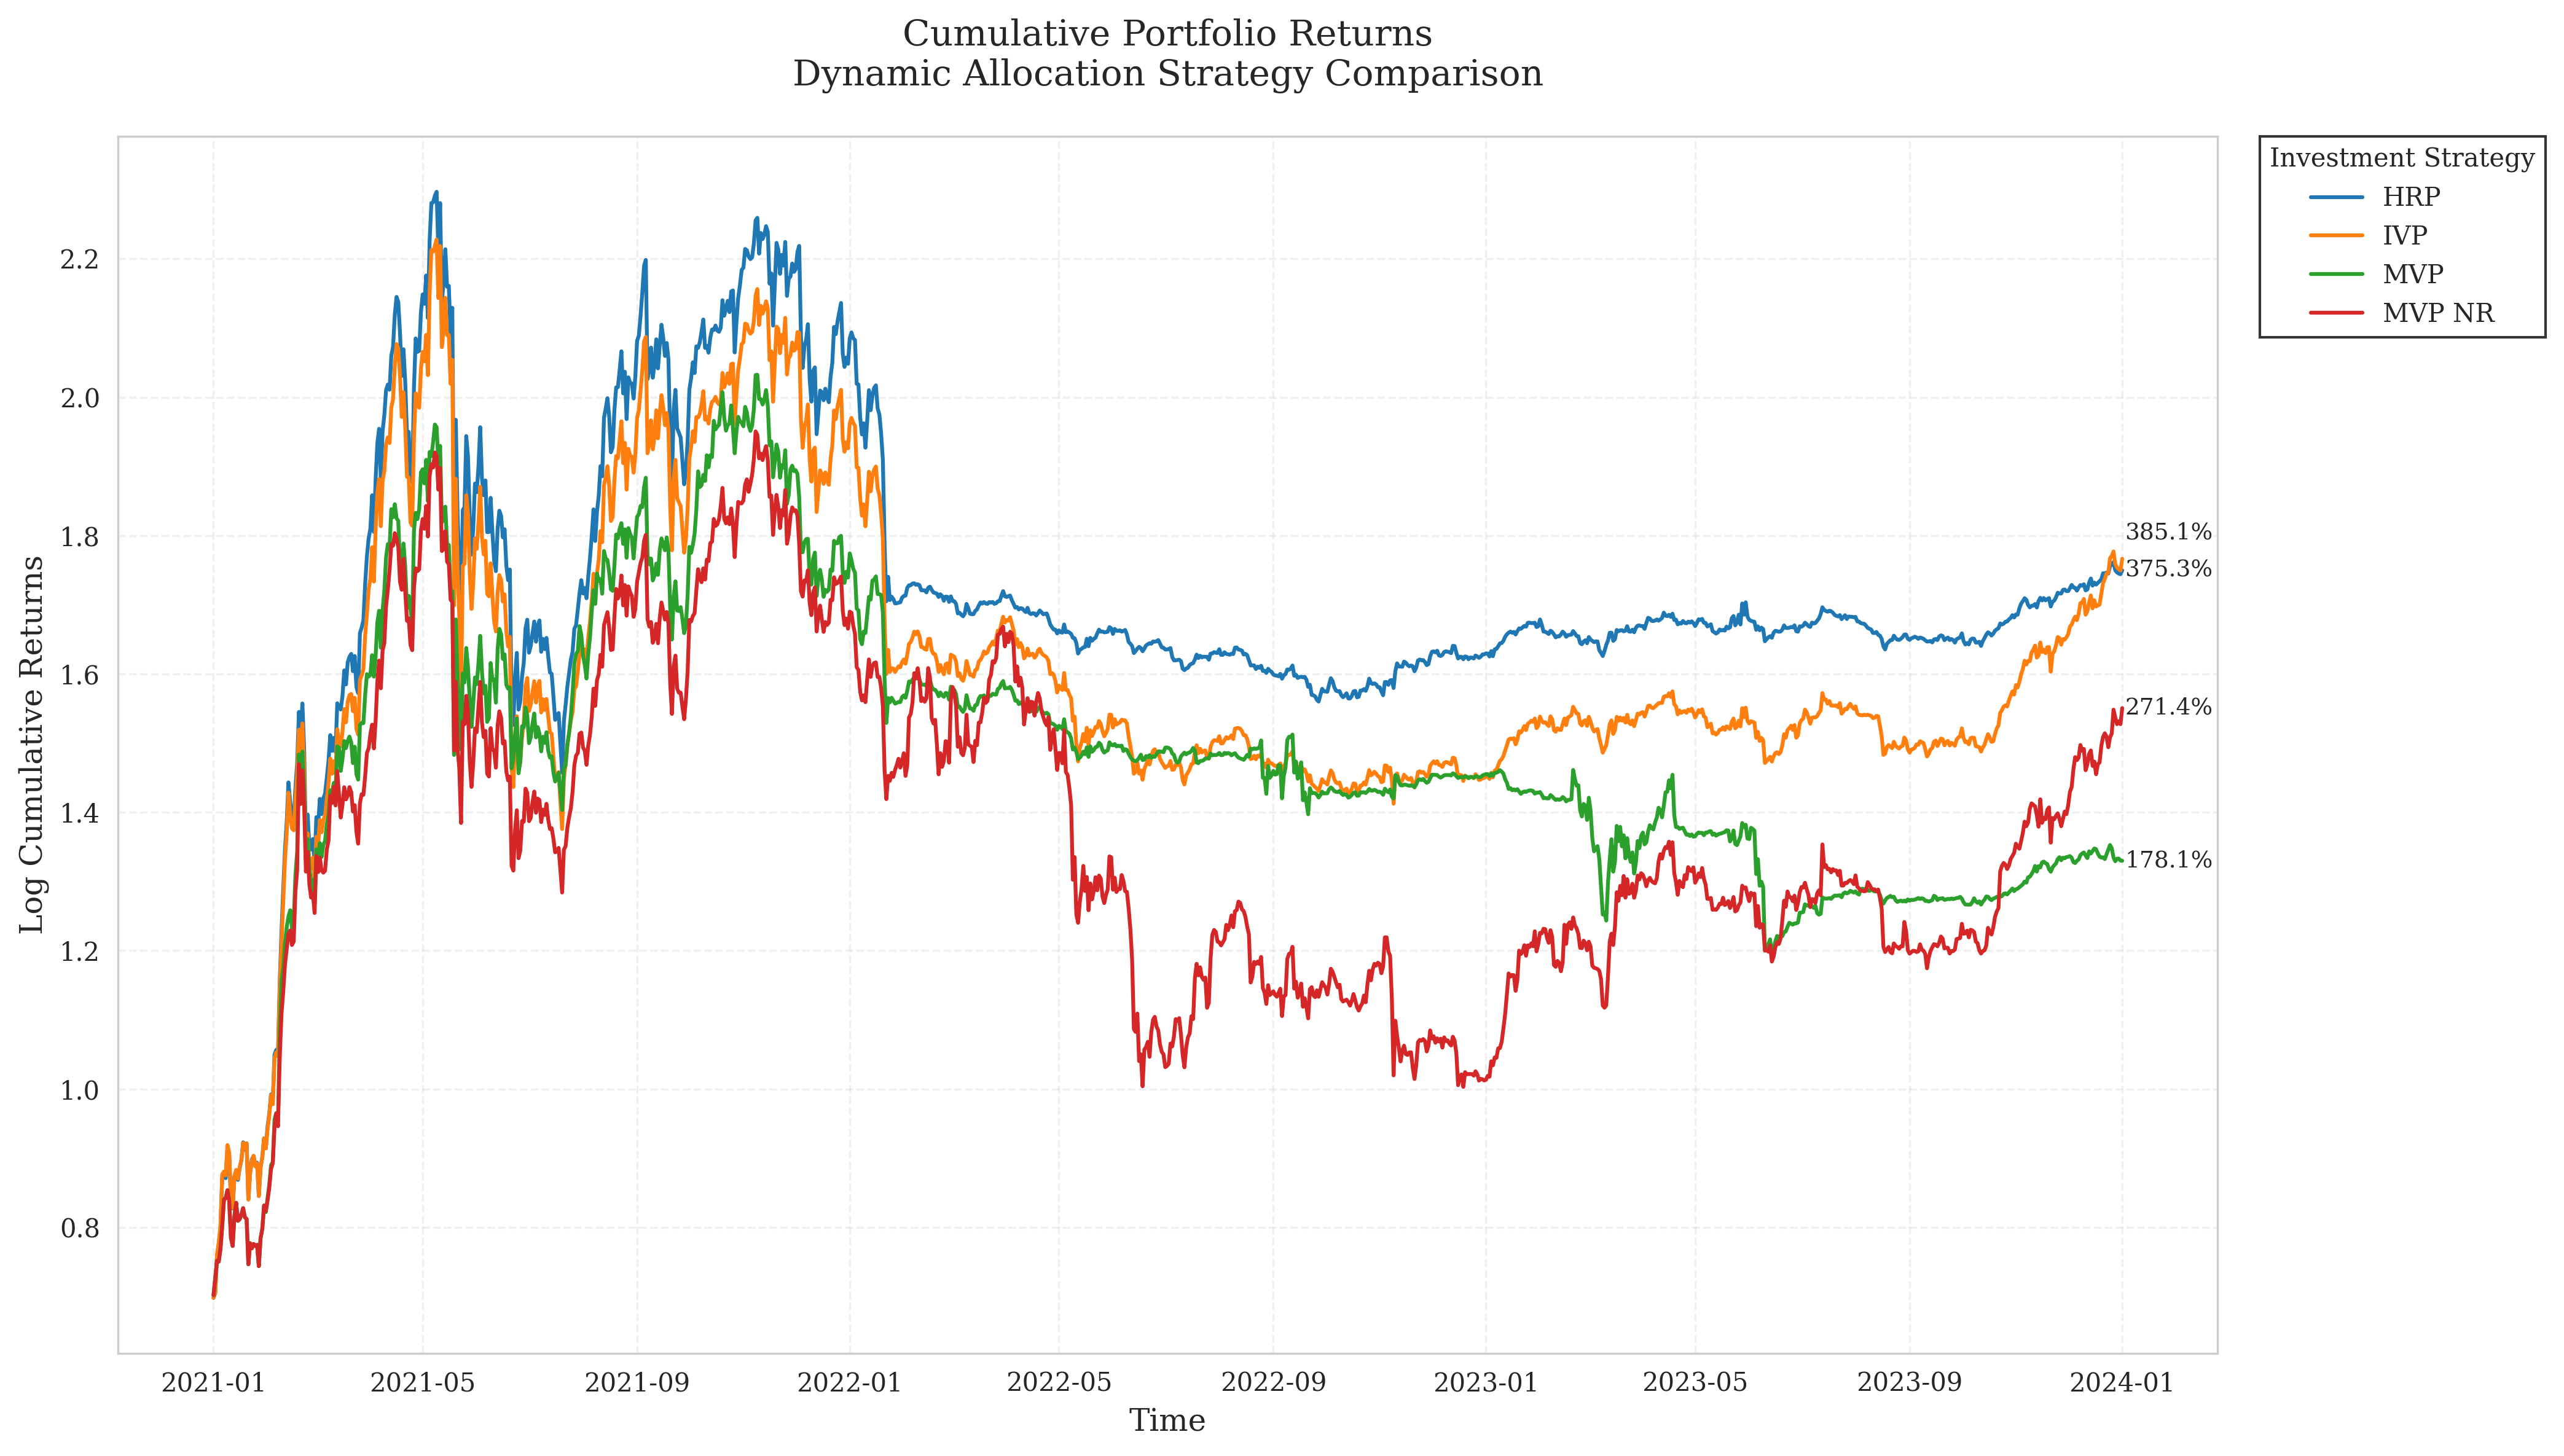
\includegraphics[width=0.7\textwidth]{rebalancing_cumulative_returns.png}
    \caption{Cumulative Returns for Weekly Rebalancing.}
    \label{fig:rebalance_cum_returns}
\end{figure}

\begin{figure}[h]
    \centering
    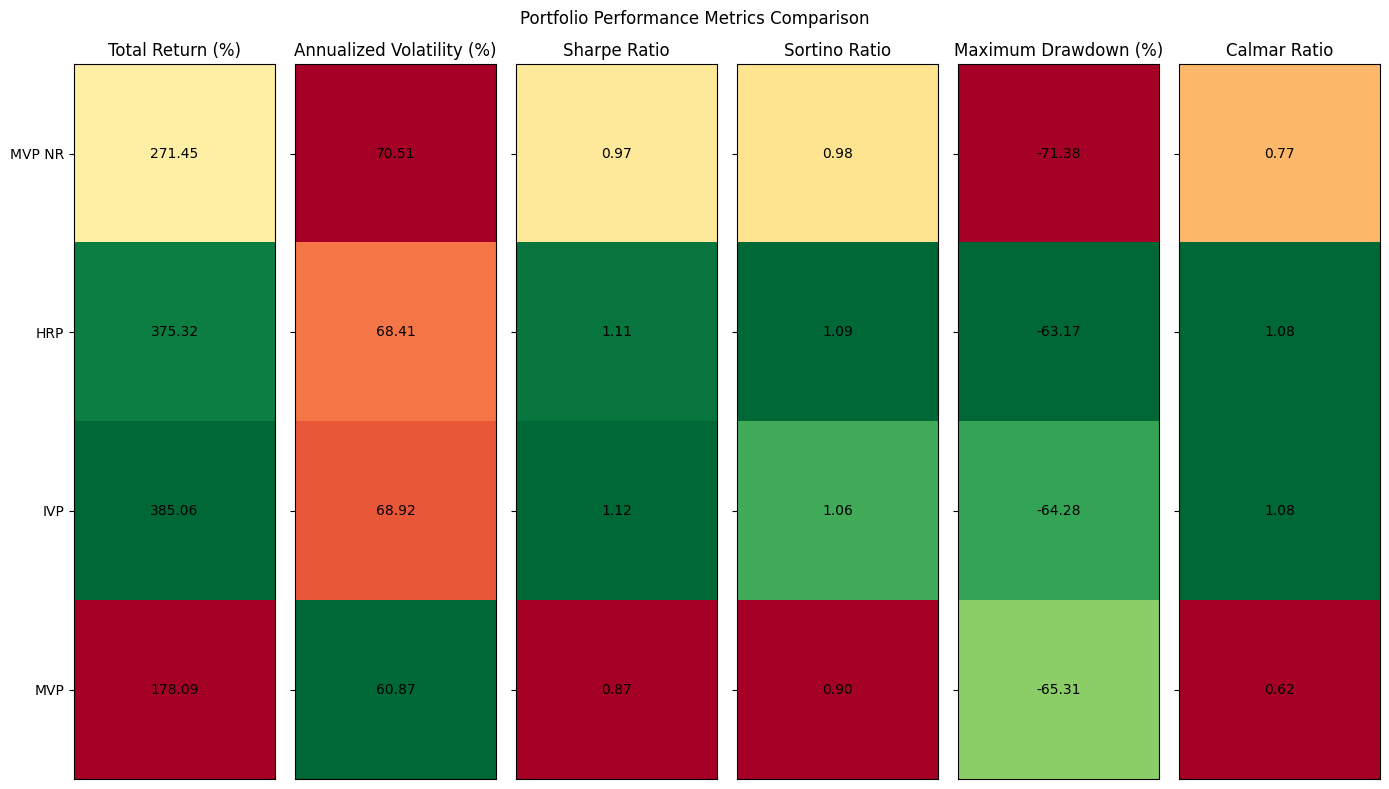
\includegraphics[width=0.7\textwidth]{rebalancing_metrics_evaluation.png}
    \caption{Metrics Evaluation for Weekly Rebalancing.}
    \label{fig:rebalance_metrics}
\end{figure}

\vspace*{.25cm}

\section{Conclusion \& Future Research}

\subsection{Conclusion}

\textbf{Diversificación}: In the case of portfolios without rebalancing, the capital allocation is more evenly distributed. However, for the scenario with rebalancing, the opposite occurs, leading to more concentrated allocations over time.

\textbf{Rebalanceo}: In the MVP strategy, each rebalancing step can lead to significantly different asset allocations. This results in high transaction costs, which reduce net returns.

\subsection{Future Research}

\textbf{Denoising}: Addressing noise caused by very small eigenvalues in the correlation matrix to improve estimation stability.

\textbf{Denoting}: Adjusting for correlation shocks by filtering out market-wide movements where all assets move in the same direction.

\section*{Acknowledgements}

We want to thank all the Ucema Quant Course professors and staff, especially Manuel Maurette, Emiliano Delefau, and Pablo Martín Gechidijian. Finally, we extend our gratitude to **Marcos López de Prado** for all the knowledge shared in his bibliography on this subject.

\section*{References}

\begin{thebibliography}{9}

\bibitem{lopez2016}
López de Prado, M. (2016). \textit{Building Diversified Portfolios that Outperform Out-of-Sample}. Journal of Portfolio Management. \texttt{https://doi.org/10.3905/jpm.2016.42.4.059}.

\bibitem{lopez2018}
López de Prado, M. (2018). \textit{Advances in Financial Machine Learning}. John Wiley \& Sons.

\bibitem{lopez2020}
López de Prado, M. (2020). \textit{Machine Learning for Asset Managers}. Cambridge University Press.

\end{thebibliography}

\end{document}
